\documentclass{article}
\usepackage{tikz}
\usetikzlibrary{calc}

\begin{document}

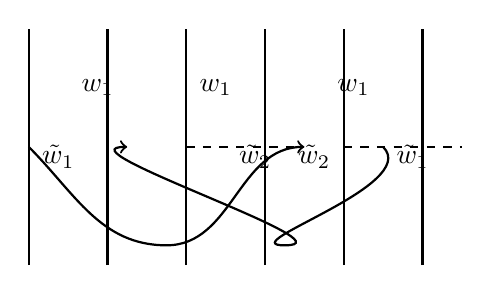
\begin{tikzpicture}[line width=0.8pt,scale=0.5]

% Draw the main vertical lines
\draw (0,0) -- (0,6);
\draw (2,0) -- (2,6);
\draw (4,0) -- (4,6);
\draw (6,0) -- (6,6);
\draw (8,0) -- (8,6);
\draw (10,0) -- (10,6);

% Draw the horizontal lines
\draw (0,3) -- ++(0,-0.5); % Double line
\draw (2,3) -- ++(0,-0.5); % Double line
\draw (0,2.5) ++(0,-0.5) -- ++(0,-0.5); % Double line
\draw (2,2.5) ++(0,-0.5) -- ++(0,-0.5); % Double line
\draw (4,3) -- ++(0,-0.5); % Single line
\draw (6,3) -- ++(0,-0.5); % Single line
\draw (8,3) -- ++(0,-0.5); % Single line
\draw (10,3) -- ++(0,-0.5); % Single line
\draw (4,2.5) ++(0,-0.5) -- ++(0,-0.5); % Double line
\draw (6,2.5) ++(0,-0.5) -- ++(0,-0.5); % Double line
\draw (8,2.5) ++(0,-0.5) -- ++(0,-0.5); % Double line

% Draw the labels
\node at (0.75, 2.75) {$\tilde{w}_1$};
\node at (4.75, 4.5) {$w_1$};
\node at (9.75, 2.75) {$\tilde{w}_1$};

% Draw the curved lines for skip connections
\draw[->] (0,3) to [out=-45,in=180] (3.5,0.5) to [out=0,in=180] (7,3);
\draw[->] (9,3) to [out=-45,in=180] (6.5,0.5) to [out=0,in=180] (2.5,3);

% Draw the dashed line for transpose operation
\draw[dashed] (4,3) -- (7,3);
\draw[dashed] (8,3) -- (11,3);

% Add the labels for the skip connections
\node at (1.75, 4.5) {$w_1$};
\node at (8.25, 4.5) {$w_1$};
\node at (5.75, 2.75) {$\tilde{w}_2$};
\node at (7.25, 2.75) {$\tilde{w}_2$};

\end{tikzpicture}

\end{document}